% !TeX spellcheck = en_US 
\chapter{Forensic audit and its computer support}


%\komentar{na zacatek shrnout co vsechno obsahuje tato kapitola. asi tak takhle:}


In this chapter we define the term "forensic audit" and other related therms to give insight into the field. Next an overview of frequently investigated types of crimes is given. We demonstrate typical roles and outline the process of forensic audit. 
%\komentar{az bude kapitola dopsana, zkontrolovat, zda toto odpovida} 

%\section{Matters of forensic audit}
%\komentar{nelibi se mi, pridat do jinych casti a zrusit}
%Forensic audit is a specialization within a field of accounting that examines and evaluates evidence concerning unproven statements for possible use as evidence in court. Forensic audit is usually used in case there is a suspicion in certain company there is a crime being committed. The background of the investigated case is rather diverse. A customer can be, for example, a CEO  who wants to examine the functioning of one of the sub-divisions of a controlling company. There can be a suspicion of some fraudulent activity or the need of forensic audit can be closely unspecified.

\section{Definition of forensic audit}\label{FA_definition}
The term "forensic" can be defined in several ways. According to merriam-webster dictionary, \cite{merriam-forensic} the definition is "relating to the use of scientific knowledge or methods in solving crimes". The term "audit" is explained in the same dictionary as "a complete and careful examination of the financial records of a business or person" \cite{merriam-audit}.

The essence of forensic audit is discovery and investigation of fraudulent intentions and fraudulent behavior. 

Forensic audit is often mistakenly interchanged with financial audit. The objective of financial audit is to verify whether financial statements are fairly stated in accordance with accounting standards. Financial auditors search for material errors or other misstatements in the accountancy.

On contrary to financial audit the ultimate goal of forensic audit is to examine existing or gained suspicion and procure evidence concerning possible fraudulent behavior. Deceptive scenarios are discovered in the process of forensic audit and evidence together with a documentation that is usable for a subsequent course of action is gathered. As a matter of principle, forensic auditors are not expected to express their opinion on guilt or innocence of suspects.


%====================================================================================
\section{Specializations in forensic audit}
Forensic audit has already been defined in \ref{FA_definition}. Noteworthy specializations include following terms.%However, there are several related specializations that can also be useful to know when dealing with this field.


\paragraph{Forensic Sciences} methodologically correctly apply a broad spectrum of scientific disciplines in order to answer questions relevant to a legal system. \cite{kyfranke} An aggregate of these sciences is sometimes also called simply forensics. Forensics is mainly used to deal with previously committed crimes or to prevent similar crimes from happening.


\begin{figure}[h]
	\begin{center} 
	%\missingfigure{Obrazek demonstrujici forenzni audit.}
	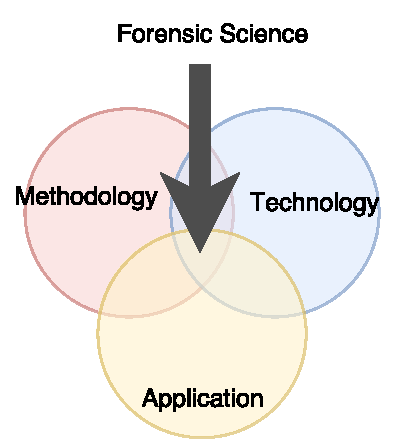
\includegraphics[width=0.4\textwidth]{img/forensic_science.pdf}
	\end{center}
	\caption{Forensic sciences}
\end{figure}

%====================================================================================
\subsection{Computer (Digital) Forensics} Computer forensics, alternatively called digital forensics, is a discipline that investigates digital evidence. It is used for recording, safeguarding, extracting and documenting evidence from various kinds of hardware. Examples of digital forensics subbranches are mobile forensics, life-system forensics, file-system forensics, network forensics and multimedia forensics. 

Digital evidence can be retrieved from plenty of digital equipment that are able to store usable pieces of information. These include not only computers, mobile devices, (smart) phones, (surveillance) cameras, PDAs etc., but also for instance copy machines, cars, washing machines or houses. This is a correlative of the Internet of Things (IoT) which is currently an emerging trend in technology. Common digital data used as an environment to search for evidence could include, for example, disk image of a device, a memory image of a device, NetFlow data, complete network communication, or even parts of log files gained from the service provider. 

Digital data are created mostly when working with digital equipment. When using the RAM (Random Access Memory),  programs regularly leave traces such as variables and input/output data. The user also saves various kinds of data when saving documents and sending emails etc.. This kind of data remains in the memory and can be a source of evidence. For example, it is possible to trace the sending of an email in several instances such as in the browser, on the web page presence of an attachment is recognizable, the email is traveling via the network and the provider running the service has a log about the email. Having adequate authorization, such as the police has, it is possible to request a record about any activity from the provider.

The data in computer memory is divided into several groups. Volatile data are temporary data that is not permanently saved. Data available to users, typically files, are called active data. Meta-data are pieces of information about data. It typically consists of facts concerning the format of data, the time of creation etc.. Using meta-data of a picture as an example, it can store the time that was set in the device when the picture was created, facts concerning the location, the focus distance, the exact name of the camera and possibly other details. Similarly, in case of an document the facts concerning the time and the user who created the document can be found in the meta-data of the data. System logs are another type of data, where, for example, an facts concerning how the system is running, is provided. The purpose of these logs is to make a potential problem easier to find and resolve. Among other things, the system log monitors the activity of the user. Temporary files are files providing auxiliary space. Typically, the .tmp file extension is used and the file is used for saving intermediate results. Another type of data that can be found in computer memory is residual data. It is, in fact, a listing of the memory, the entity of unallocated memory, parts of files, deleted but not overwritten files and other pieces of memory.

%To be able to analyze the meaning of the data we need tho know their format.

Forensic analysis of digital data deals with searching for evidence in the field of information technology, their interpretation and presentation. The basic requirements are to find the desired evidence in a way that the methods are repeatable and the results are unquestionable. Forensic analysis always adopts an unbiased stance on the result.

First step in preparation of the data is its extraction from the device. These extracted data are also called "best evidence". Immediately after that the data is hashed and another copy of the data is made for processing purposes. This is important in case a change in the working copy is made while processing the data, the hash can always be easily check to verify the correctness of the data. It is important to document the procedure of extraction while extracting. It is possible, for example, to add a new entry to a log file, but it must be well documented to prevent any future mistakes.


%====================================================================================
%\komentar{
%
%postup: extrahovat data - bitova kopie, pokud pracujeme s orignalnim zarizenim, je potreba dokumentovat veskery posutp aby bylo dohledatelne, ktere zmeny jsme udelali napriklad pri extrahovani dat. kontrola autenticity pomoci hashe abychom si mohli byt jisty ze data nebyla zmenena
%
%tato primarni data = "best evidence"
%
%analyza dokumentace vychoziho stavu!, co mame najit? kde mame najit? do kdy to mame najit?
%neni univerzalni postup
%data carving, predzpracovani dat
%
%znalosti nastroju +znalosti fungovani systemu
%
%interpretace vyhsledku - casova osa
%
% 	
%zminit jak se obecne obnovuji data? (princip)}
%====================================================================================

\subsection{Computational Forensics} Computational Forensics is an research domain that uses the means of computational methods to study any kind of evidence. Computational forensics involves modeling, computer-based \nohyphens{analysis,} computer simulations etc.. This specialization uses methods such as machine learning, data mining, image processing, statistical pattern recognition, fuzzy logic or data visualization to discover any hidden forensic knowledge. 

%%================================================================================
%\section{Selection of specific techniques or tools used in forensic audit}
%\paragraph {Data mining}
%
%\paragraph {Fuzzy logic}
%
%\cite{stoffel2010fuzzy}
%
%\paragraph {Machine learning}
%
%\paragraph {}
%
%
%
%\komentar{
%
%
%
%
%co nas zajima - situace, kde je vhodne uvazovat pocitacovou podporu
%pocitacova podpora muze mit mnoho druhu-
%vyuzivani konkretniho SW 
%	analyticky, 
%	statisticky, 
%	podpora projektoveho managementu
%	nastroje na sdileni informaci pri praci na projektu
%vyuzivani nekterych obecnych principu 
%	ctj. fuzzy logika,
%		
%	ctj data mining
%		analyzovani zaznamu konverzaci,
%		analyzovani vztahu mezi lidmi / chovani 
%	strojove uceni?
%	tyto principy mohou byt zakomponovane v nekterych konkretnich SW nastrojich vyse
%vyuzivani konkretnich znalosti v pripade ziskavani dat z hw
%	znalosti o fungovani operacnich systemu obecne
%	znalosti o sitich
%	konkretni znalosti o ukladani dat na disk
%	tyto veci mohou slouzit jako nastroje na ziskani dukazu.
%
%zdroje dat / dukazu
%	zpracovatelne pomoci pocitace
%		vypisy z uctu/ ucetnictvi, verejne databaze vlastnictvi, socialni site, elektronicka komunikace z dostupnych zdroju, znalosti / fakta o konktetnich osobach...
%	nezpracovatelne pomoci pocitace, nebo vyuzivajici specificke principy sveho vlastniho oboru
%		tady myslim sbirani otisku prstu a podobne oblasti, ktere resi specialiste
%
%
%
%}
%
%
%%================================================================================



\paragraph{} The subbranches of digital forensics as well as the specializations of computational forensics play their own part in the investigation of complex cases. They are used to provide intermediate results for the investigation by answering closely specified questions. Some of these methods can also be used indirectly as functionalities provided by a software that is used in the investigation.  

%====================================================================================
\seda{
\section{Existing software analysis}

The existing software in the market is either inefficient in terms of results or does not full fill the requirements for conducting proper evaluation. For this reason, Computer Forensic Tool Catalog has been created as an effective way of connecting practitioners to the tools they need. This catalog is available on the "National Institute of Standards and Technology" web pages \cite{10}. The information about forensic functionalities and associated technical parameters and their values can be provided by any vendor, in order to be integrated to the database. All tools are being reviewed before posting. This catalog can be considered rich in the database and it is also systematic and searchable. The only problem is it is not possible to select free tools only. This catalog can be recommended to any practitioner as a useful instrument for choosing suitable software for their situation. Although other lists of software can be found browsing the Internet, this one is reliable and provides the possibility of search in the tools according to technological needs.

The functionalities of the tools contained in the catalog are mostly usable in one of the first stages of forensic audit. This stage could also be called preparatory stage because the auditor is preparing background for the search for evidence. Documents and all possibly available data related to the studied case are being collected. Depending on the character of the case, data from various pieces of hardware can be collected. In some situations, if the tool is sophisticated enough, the following analysis of the data can be performed immediately within the same tool.


The work of the auditor usually starts by getting to know the situation because each case has its specific character. After that they need to collect all the hardware that holds important data and extract all the data stored in these devices. According to the type of device they may use proper software that is good for acquisition of the data stored.


%//pridat tabulku reprezentujici: platformy, cena, funkce(), specifika, reprezentace dat, jak moc jsou bezne vyuzivane

\paragraph{Quantative software}\label{qSW}

Specialized fraud identifying software is making a passage into the business, with extortion module discharges from both ACL and IDEA\textsuperscript{\textregistered}, extortion parts in SAS and SPSS, and a devoted extortion discovery program in Picalo. Programming organizations like ACL and IDEA\textsuperscript{\textregistered} give exercise manuals that can be utilized as a part of courses, however, these exercise manuals have couple of illustrations of direct misrepresentation recognition particularly with cutting edge procedures. Approaches like the theory testing methodology are an initial phase in giving procedure research, immense extra research—both observational and field—are expected to approve and augment the current ideas.

Quantative software organizations give complete preparing on measurable programming and systems. The two driving programming bundles are EnCase by Guidance Software and the Forensic Toolkit (FTK) by Access Data . These suites give shorter expectations to absorb information than past utilities and convey a more prominent number of experts to the field more rapidly. Both bundles give tasks positioned procedures to securing and illustrating forensic information.


Lately, Linux based apparatuses have been prevalent as free distinct options for the conventional suites. Helix, the Penguin Sleuth, and Security Tools Distribution are Linux dispersions that run specifically from CD, giving clean situations to seeking a PC without the requirement for cloning (Causey, 2005). These instruments boot a suspect PC straightforwardly to Linux and mount the client hard drives in read just mode, basically bypassing most passwords and security insurances. While Linux based instruments are more hard to use and do not have the same point of reference in court as EnCase and FTK, they have to be well known with a few evaluators.


%TODO: poradne popsat qSW

\paragraph{The R Project for Statistical Computing} 
R is mathematical software specialized in statistics. It concerns an open-source implementation of the S language, which is used by other professional statistical applications. It is a good choice in case that great amount of data needs to be processed because R is suited for large data sets.
%\cite{http://www.r-project.org/about.html}


\paragraph{Using SAS to evaluate risks }

Measurable packages like SAS and SPSS give full drifting modules to the intrigued inspector. Statement on Auditing Standards (SAS) and consideration of fraud in a financial statement audit requires inspectors to evaluate the risk that misrepresentation might physically misquote budgetary articulations. Regardless of SAS 99 being an imperative necessity towards expanded misrepresentation, a study by "Marczewski and Akers"\cite{21} uncovered that Certified Public Accountants (CPAs) do not envision that SAS 99 will generously expand review viability. Another study found that while SAS 99 expanded examiner obligation, most reviewers experienced issues recognizing the work and its risks.



\paragraph{SPSS for statistical and analytical services}

SPSS is one of the leading analytical instruments. It provides statistical and analytical services the abbreviation originally meant Statistical Package for the Social Sciences. This software supports areas of social survey and market research, predictive and advanced analytics, decision management and deployment or predictive solutions.

%\cite{http://www-01.ibm.com/common/ssi/cgi-bin/ssialias?infotype=PM&subtype=BR&appname=SWGE_YT_YV_USEN&htmlfid=YTB03015USEN&attachment=YTB03015USEN.PDF}

\paragraph{COFEE}
Useful tools for basic forensics are Microsoft's COFEE tools. They are a set of PC forensic and evaluating tools that Microsoft puts on a USB key and provides for law requirement. It is used in attempting to concentrate information from a PC. There was some apprehension that it was an "indirect access", however, individuals demanded it was no such thing, yet only a gathering of essential tools. Still, the this framework was advanced as being valuable for decoding passwords and examining a PC's information and web action that appeared to be alarming. If Microsoft was giving it out to law requirement, it appeared to be likely that others would have entry to it also.


%doplnit!
\paragraph{IDEA\textsuperscript{\textregistered}}
IDEA\textsuperscript{\textregistered} is an effective and easy to understand information investigation tool intended to help reviewers; bookkeepers and other account experts perform information examination rapidly to help enhance reviews and distinguish control breakdowns. It permits to dissect 100\% of the information to ensure information trustworthiness and gives simple investigation more that 100 major studied activities. 

At the point when the information originates from distinctive sources and in a mixed bag of configurations, information investigation can infrequently be a test. The capacity to import different information sets and represents it as if they were one that lets us to see the master plan. We have the capacity to recognize connections, examples and inconsistencies and additionally direct a far reaching examination of value-based information. 

Import Data from Practically Any Source IDEA\textsuperscript{\textregistered} permits us to rapidly import a boundless measure of records from for all intents and purposes of any source, including spreadsheet and \textbf{database programming}, mid-extent bookkeeping projects, ERP frameworks, legacy centralized servers, telecommunication switches, travel and costs applications, level and printed documents, for example, PDFs, plain content (.txt), and print-report (.prn) records. Rearranged analysis instead of programming macros can use more than 100 review particular undertakings that easily search for copies, identify dumps in numeric groupings, group information by classes and channel various lines and sections of data in seconds. IDEA\textsuperscript{\textregistered} permits us to record each investigative step and reuse for future utilization, through a graphical interchange and customized interface. 

\paragraph{Microsoft Analytics Services}
Procedures utilized for misrepresentation discovery fall into two essential classes: factual systems and computerized reasoning. Examples of measurable information examination methods are: 

\begin{itemize}
\item Data preprocessing strategies for discovery, acceptance, slip adjustment, and topping of missing or off base information.
\item Calculation of different factual parameters, for example, midpoints, quintiles, execution measurements, lihelihood circulations. For instance the midpoints may incorporate normal length of call, normal number of calls every month and normal defers in bill installment.
\item Models and likelihood dispersions of different business exercises either regarding different parameters or likelihood circulations.
\item Computing client profiles.
\item Time-arrangement investigation of time-ward information.
\item Clustering and grouping to discover examples and relationship among gatherings of information.
\item Matching calculations to recognize abnormalities in the conduct of exchanges or clients when contrasted with already known models and profiles. Methods are likewise expected to dispose of false alerts, assessment chances, and foresee eventual fate of current exchanges or clients. % \todo cite.
\end{itemize}


}
%====================================================================================



\section{Types of investigation}

Forensic auditor can be asked to investigate really wide range of types of situations. Basically any kind of suspicion on potentially bad behavior can be an impulse for investigation. However, not all kinds of crimes are of our interest. For example violent crimes, cash theft, assault, robbery, rape, actual bodily harm and similar crimes are rather part of a detective work. Forensic auditors typically do not deal with such crimes. 

On the contrary, fraudulent crimes are those ideally fitting for forensic investigation. There are many different kinds of fraud that forensic auditors deal with. To provide an overview of the wide range, these frauds can be classified into following three groups: corruption, asset misappropriation and financial statement frauds. These frauds are the most frequently investigated scenarios.

\paragraph {Corruption}
Corruption can be characterized as a misuse of status. The motivation behind corruption is a desire to gain money, material possession or other advantages. By extension an involvement in a corruption relationship is a sign of moral and ethical failure of individuals. Several specific kinds of corruption are bribery, acceptance of a bribe, extortion, misuse of power, misuse of information or conflicts of interest. Research shows that corruption is involved in around one third of all frauds. \cite{weaver}

\paragraph{Bribery} is an unauthorized advantage in form of recipient's behavior alternation in exchange for money, goods or other forms of recompense. On contrary to bribery extortion occurs when money or some action is demanded in order to secure particular outcome. Conflict of interest and misuse of power or information can be categorized in one group. In such situations fraudsters use their power to achieve personal profit without regard to their position responsibility. Consequently their behavior negatively influences the company which is giving them their power. For example a manager of local division of a company choose his friend to be the paper supplier even though that his price is significantly much higher than the price of other paper suppliers.


\paragraph {Asset misappropriation}
is the theft or embezzlement of company assets by directors, other fiduciaries or employees. Is by far the most common economic crime experienced by organizations reporting any fraud, with 69\% of respondents suffering from it. \cite{pwc-asset} It happens when people who are entrusted to manage the assets of an organization steal from it. The stealing usually starts small and when perpetrators gain their confidence it becomes bigger. In consequence of this asset misappropriation can be a serious problem and can cause immense losses. 

The specific kinds are cash theft, inventory theft or using company assets for personal purpose. Special sort of asset misappropriation is fraudulent disbursement, i.e. for example fictional billing or raising an invoice that is not in compliance with the field of the supplier's enterprise. An interesting particularity is that asset misappropriation is far more likely to be committed by individuals than by a group of perpetrators\cite{whitepaper}.


\paragraph {Financial statement fraud}
This kind of fraudulent activity is based on deliberate falsification of accounting records. It can include manipulation with expenses, manipulation of revenue figures, overstating assets or improper disclosure. This is regularly done to give the budgetary proclamations a specific inclination, for instance covering liabilities to enhance any examination of liquidity.

%\section{When to use forensic audit}
%\komentar{asi spis nez priklady popsat za jakych situaci...}
%\sediva{\blindtext}
\anglictina{dilci otazky}

\paragraph{} Aside from investigations mentioned above forensics can be also used to help solving partial questions found in the process of investigation. Similarly in case of need to deal with partial issues such as file recovery a specialist in forensics might be asked for help.

%====================================================================================



\section{How to prepare for a forensic audit}
%\komentar{v hrubych rysech jak to probiha (to co uz mam sem patri), na zaklade toho, co jsem zjistila, FA funguje takto:...\\}

On the basis of what we have found the process of forensic audit works as follows. When it is decided that certain situation will be investigated in forensic audit it is important to prevent all investigated individuals to access all related documents and electronic evidence. It is also recommended to limit their access to corporate information systems. 

Next step is to formulate properly the assignment. To define the extent and expectations on the outcome of forensic audit. To prevent a misunderstanding the assignment should be as specific and detailed as possible. It is best to choose the right audit company according to references and their experience with similar cases as the one we have specified.

When a client contacts an audit company with an assignment they usually schedule a meeting together, formulate sign and accept the assignment. The ordering party should be prepared to provide access to corresponding electronic and paper-like documentation as well as accept the fact that auditors are going to question employees and case-related person. On the other hand the audit company undertakes to refrain from sharing all the confidential information with third parties.A team of specialists that are convenient to the assignment is formed and the inspection is launched. 

In some cases the extent of the order is quite complex such as investigation of processes in one separate division of a company or investigation of complex corruption crimes. Nevertheless there may also be much easier cases where the audit firm is asked only to recover certain documents, or to examine particular piece of hardware. 

The following steps of precise methods of forensic audit are not definite. The ability to adapt in new situations is one of many essential capabilities for the team of forensic auditors. The variety of investigated cases is so vast that there is no universally valid and precise course of action in the same time. Therefore on this place we present only general methodology of forensic audit. Several selected methods of forensic audit will be described later in this document. \komentar{link na spravne misto!}

\section{General methodology of forensic audit}
In this section we present basic phases that are used while performing forensic audit. This process is most commonly divided into four stages: Accumulation, Examination, Analysis and Reporting. This basic methodology starts after the  selection of the audit company and after the specification of the assignment; at the same time when the real work of forensic auditors begins.

\begin{figure}[h]
	\begin{center} 
	%\missingfigure{Obrazek demonstrujici forenzni audit.}
	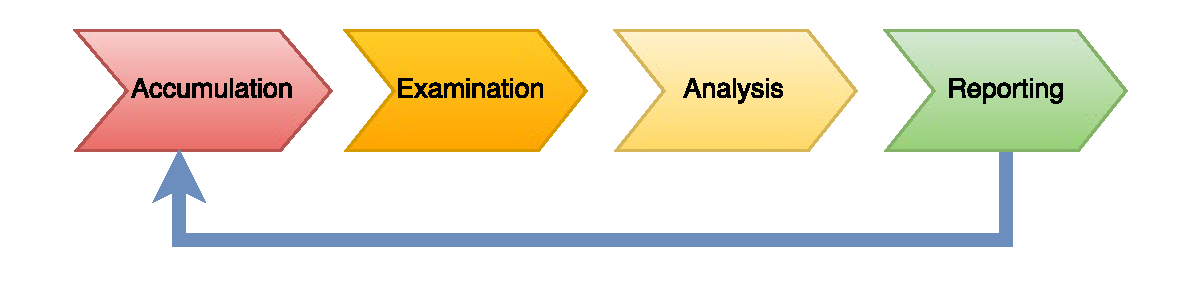
\includegraphics[width=1.0\textwidth]{img/general_methodology.pdf}
	\end{center}
	\caption{General methodology of forensic audit}
\end{figure}

%vvvvvvvvvvvvvvvvvvvvvvvvvvvvvvvvvvvvvvvvvvvvvvvvvvvvvvvvvvvvvv
\paragraph{Accumulation:} 
The main purpose of this stage is to acquire as much usable data as possible. It means recognize possible sources of data and provide backup record. All the sources of data and information, including necessary cross examination and other sources of evidence, should be utilized in this phase. All the information from the conceivable sources of pertinent information should be gained.

\paragraph{Examination:}
Examinations include forensically preparing all the gathered data. This can be done using a blend of computerized and manual systems to survey and concentrate specifically compelling information. 

\paragraph{Analysis:}
The following period of the procedure is to investigate the consequences of the examination, using legitimately reasonable routines and systems. The aim is to infer helpful data that addresses the inquiries that were the impulse for performing the accumulation and examination. %\komentar{grrrrrr...}


\paragraph{Reporting:}
The last stage is reporting the consequences of the investigation, which may include depicting the activities utilized, clarifying how devices and methods were chosen, figuring out what different activities should be performed and giving proposals to change to approaches, rules, techniques, apparatuses, and different parts of the measurable procedure. 


%^^^^^^^^^^^^^^^^^^^^^^^^^^^^^^^^^^^^^^^^^^^^^^^^^^^^^^^^^^^^^^
%\sediva{\blindtext}





%===================================================================================
\section{Use case diagram of forensic audit in general}

As we see it there are three basic roles in forensic audit. A customer who wants a particular case to be investigated. The action of the customer is to assign the order to a audit company. A representative of the company i.e., for example, forensic auditor takes over the order and starts the investigation. The operations requiring specialized skills can be delegated to an expert from the proper field. Forensic auditors together with specialists then investigate the case and search for the evidence. In the end of the investigation the auditor reports the conclusion to the customer. 

\begin{figure}[h]
	\begin{center} 
	%\missingfigure{Velky obrazek vsech zainteresovanych stran - f.auditor, datovy analytik pro FA, zakaznik (zadavatel, materska spolecnost)}
	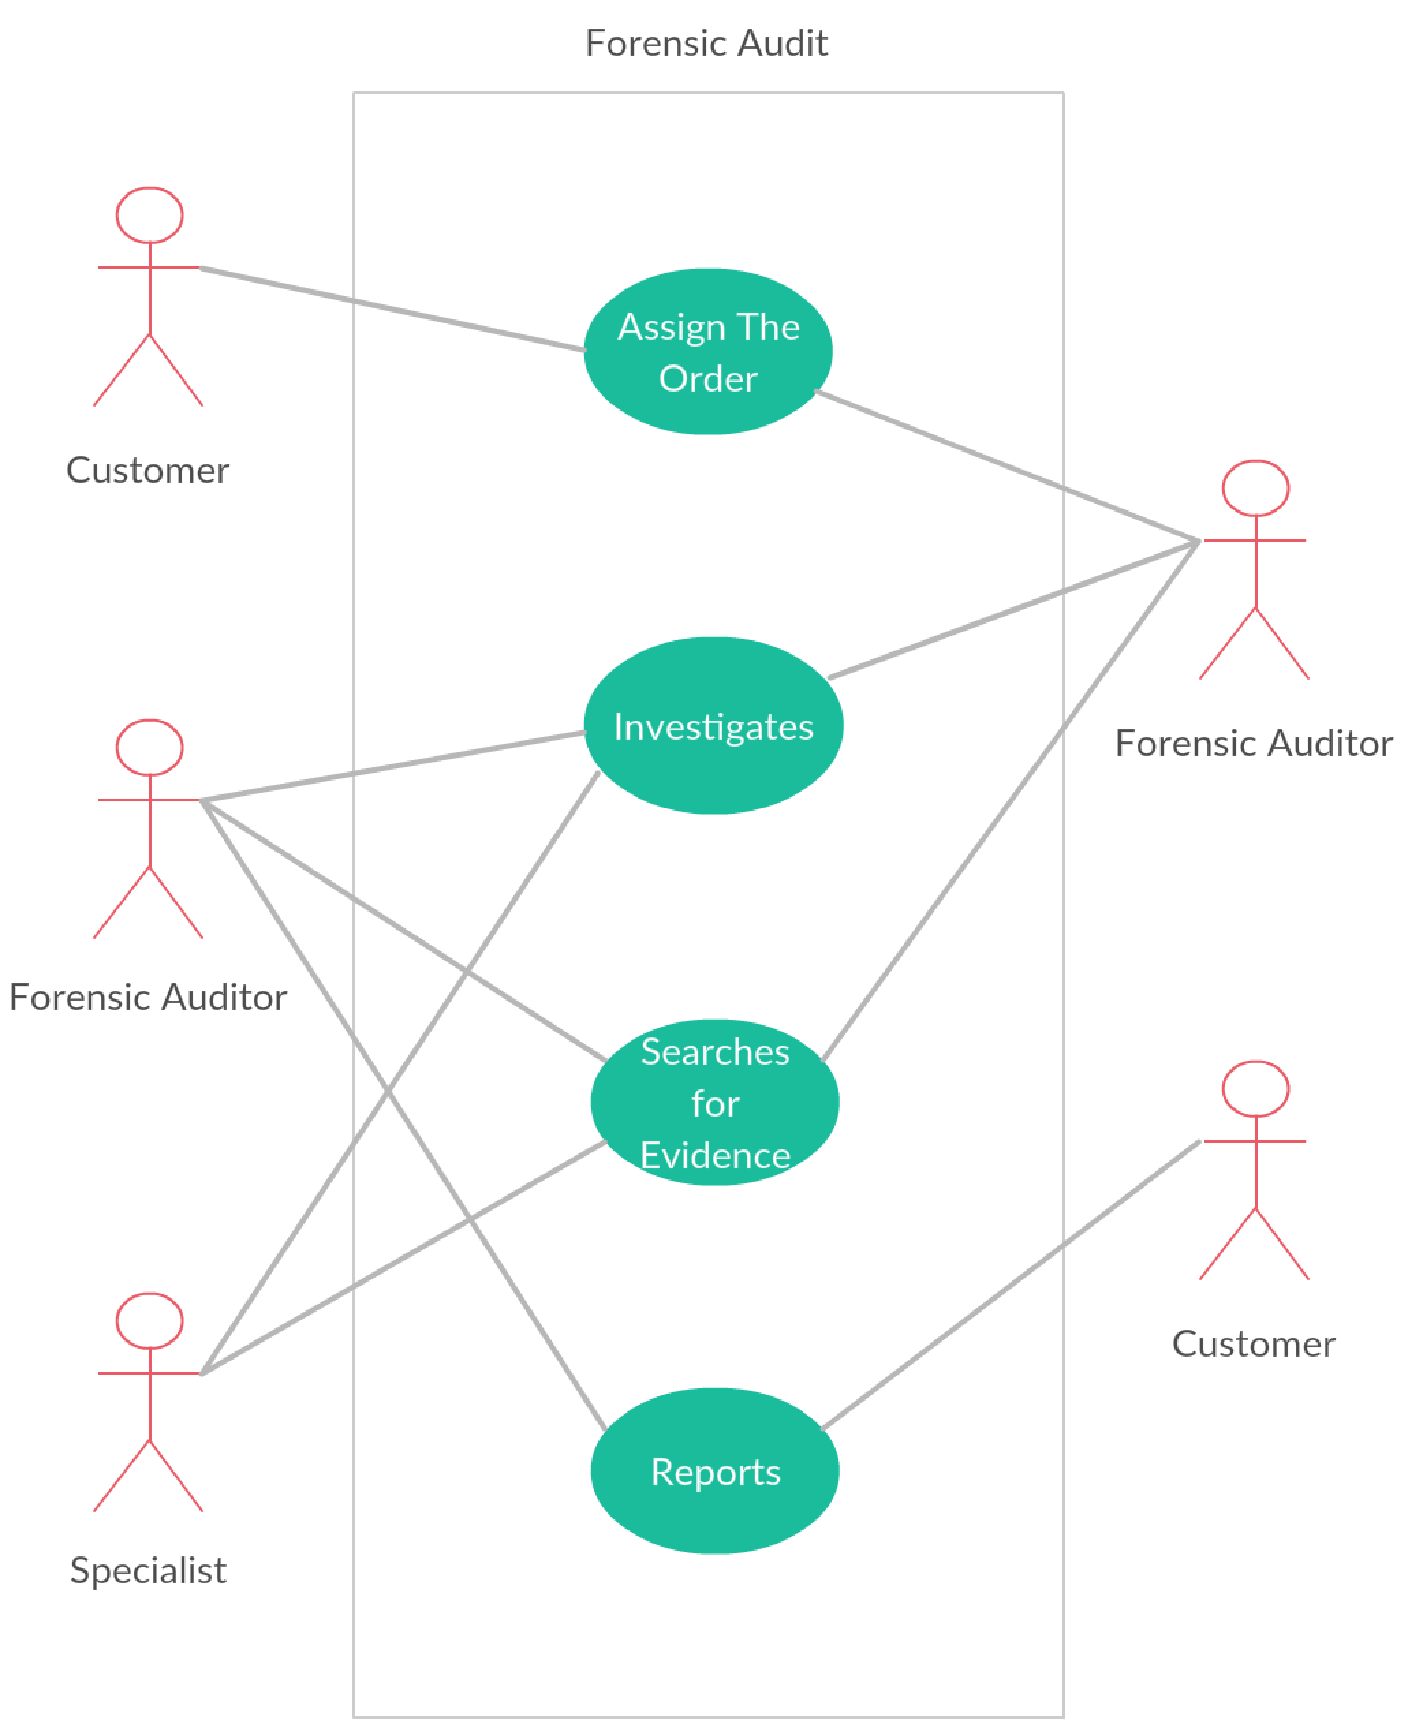
\includegraphics[width=0.8\textwidth]{img/usecase/use_case-FA_general2.pdf}
	\end{center}
	\caption{Use case diagram of forensic audit in general}
\end{figure}

%%================================================================================
%\komentar{\section{co sem jeste zahrnout:}}
%\komentar{
%	VIZE: Zbyle obecne druhy odhalovaneho chovani tak nejak rozdelit do skupin podle toho, jaky druh pocitacove podpory je obecne vyuzitelny. Pak se mozna pokusit k sobe priradit dany precin a metodu. Z metod nechci zminovat konkretni SW, ale spise obecne oblasti reseni - jak vyuzivame data mining, fuzzy logiku, strojove uceni (nebo alespon co to je a ze se take muze vyuzit), kvantitativne analyticky SW, forenzni toolkity na obnovu dat a podobne.
%}
%
%\komentar{
%Priklady
%
%·         Pan X, reditel ceske pobocky mezinarodni firmy\\
%
%o   ma bratra, ktery mu dodava papir 500 Kc za balik.\\
%
%·         Pani Y, ucetni spolecnosti\\
%
%o   zauctuje falesnou fakturu na zalevani kvetin ve vysi 20 000 Kc (s vedomim pana Novaka)\\
%
%·         Pan Z, spravce budovy\\
%
%o    zamestna na parkovou upravu pred spolecnosti firmu, ktera mu stavi rodinny dum\\
%
%Typy problemu\\
%
%·         Predrazene dodavky\\
%
%·         Fiktivni faktury\\
%
%·         Nesoulad podnikani dodavatele a faktury\\
%
%·         Paralelni spoluprace\\
%}
%%\dotaz{Z predchozi vize chci prejit v dalsi kapitole zpet k obecne metodologii a diagramu z ARISu. Nevim, jak na to plynule navazat aby to davalo celkove hlavu a patu. Snad me jeste neco napadne.}
%
%%================================================================================


